\section{Salary Dataset}
This task involved analyzing a dataset containing salary information for various employees. The objective of this task was to design a linear
regression model to fit the data and predict salaries based on years of experience. 
The model's performance was evaluated using metrics such as Mean Squared Error (MSE)~\cite{wiki_mse}, Root Mean Squared Error (RMSE), Mean Absolute Error (MAE), and R-squared (R²)~\cite{wiki_r_squared} to assess the accuracy of the predictions.

\subsection{Implementation Details}
The Linear Regression model was implemented using the \texttt{LinearRegression} class from the \texttt{sklearn.linear\_model} module~\cite{sklearn_linear_model}.
The training data was loaded from the provided CSV file using Polars~\cite{polars}. 
The features (years of experience) and target variable (salary) were extracted from the dataset and used to fit the \texttt{LinearRegression} model.

\subsubsection{Data Handling}
The dataset was read using Polars as follows:
\begin{minted}{python}
import polars as pl

data_location = 'dataset/salary/Salary_dataset.csv'
data = pl.read_csv(data_location)
X_train = data[['YearsExperience']]
y_train = data['Salary']
\end{minted}

\noindent The resulting dimensions of the feature and target arrays were:
\begin{itemize}
    \item \textbf{X\_train}: (30, 1) -- 30 samples with 1 feature (Years of Experience)
    \item \textbf{y\_train}: (30,) -- 30 target values (Salary)
\end{itemize}

\newpage
\subsubsection{Model Training}
The Linear Regression model was trained using the following code:
\begin{minted}{python}
from sklearn.linear_model import LinearRegression

model = LinearRegression()
model.fit(X_train, y_train)
y_pred = model.predict(X_train)
\end{minted}

\noindent The resulting dimension of the predictions array was:
\begin{itemize}
    \item \textbf{y\_pred}: (30,) -- 30 predicted salary values
\end{itemize}

\subsection{Results}
\subsubsection{Plotted Graph}
The resultant graph of the linear regression model is shown in Figure~\ref{fig:salary_regression}.

\begin{figure}[htbp]
    \centering
    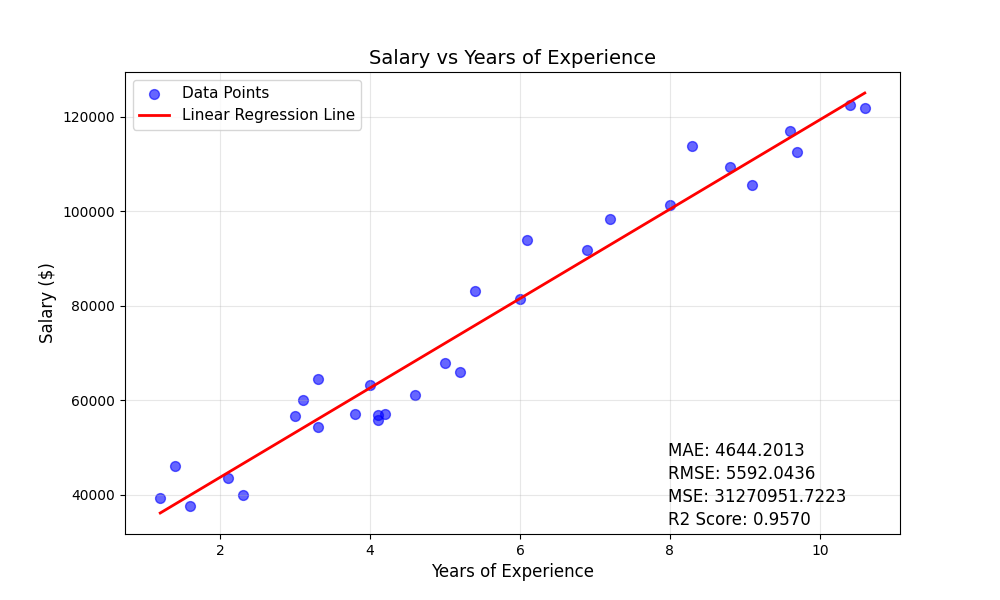
\includegraphics[width=\textwidth]{images/salary_analysis_plot.png}
\caption{Linear Regression Model for Salary Prediction}\label{fig:salary_regression}
\end{figure}

\newpage
\subsubsection{Analysis}
The performance of the Linear Regression model was evaluated using several metrics.
The results are summarized in Table~\ref{tab:salary_results}.

\begin{table}[htbp]
    \centering
    \begin{tabular}{ || l || c || l || }
        \hline
        \textbf{Metric} & \textbf{Value} & \textbf{Interpretation} \\
        \hline\hline
        R² Score & 0.9570 & Excellent model fit (95.7\% variance explained) \\
        \hline
        MAE & \$4,644.20 & Average prediction error of \$4,644 \\
        \hline
        RMSE & \$5,592.04 & Root mean squared error of \$5,592 \\
        \hline
        MSE & 31,270,952 & Mean squared error (in squared dollars) \\
        \hline
    \end{tabular}
    \caption{Performance Metrics for Salary Prediction Linear Regression Model}\label{tab:salary_results}
\end{table}

The model demonstrates great performance with an R² score of 0.9570, indicating that the linear regression explains 95.7\% of the variance in salary based on years of experience. 
The Mean Absolute Error (MAE) of \$4,644 represents an average prediction error of approximately 5.8\% from the regression line to the actual values.

The Root Mean Squared Error (RMSE) of \$5,592 is slightly higher than the MAE, indicating that most predictions are accurate, but there are some instances with larger prediction errors. 
This can be interpreted as there being a few outliers in the dataset where the actual salary deviates significantly from the predicted salary based on years of experience.